  \section[Systematized Nomenclature in Medicine Clinical Terms\\ (SNOMED CT\textsuperscript{\textregistered})]
  {SNOMED CT\textsuperscript{\textregistered}}
  \label{sec:snomedct}

  \initial{S}\textit{ystematized Nomenclature in Medicine Clinical Terms (SNOMED CT)}\
   is a comprehensive, multilingual clinical terminology that provides clinical content and\
   expressivity for clinical documentation and reporting. It can be used to code, retrieve\
   and analyze clinical data.\
   SNOMED CT was formed by the merger, expansion and restructuring of\
   SNOMED RT\textsuperscript{\ref{sec:snomedrt}}\
   and the United Kingdom National Health Service (NHS)\
   Clinical Terms (also known as the Read Codes).\
   In a nutshell, SNOMED CT consists of concepts arranged in a hierarchy, connected\
   by relationships. The International Health Terminology Standards Development Organization\
   (IHTSDO) owns and administers the rights to SNOMED CT.\\

  \noindent According to \citep{snomed_-_user_guide_snomed_2011}, there are three basic\
  components of SNOMED CT:
  \begin{itemize}
    \itemsep0ex
	  \item{Concepts}
	  \item{Descriptions}
	  \item{Relationships}
  \end{itemize}

  \subsection{Concepts}
  Concepts are clinical ideas, ranging from \emph{abscess} to \emph{zygote},\
  identified by a unique numeric identifier (\textit{ConceptId}) that never changes\
  and represented by a unique human readable \textit{Fully Specified Name (FSN)}.\
  The concepts are formally defined in terms of their Relationships with other concepts.\
  These logical definitions give explicit meaning which a computer can process and query\
  on. Every concept also has a set of terms that name the concept in a human-readable\
  way. There are well over 300,000 active concepts in the terminology with differing levels\
  of granularity linked to one another by\- \textbar ~is a \textbar \- ~relationships as depicted\
  in Figure~\ref{fig:snomedct_concepts_granularity}.\\
  \begin{figure}[!ht]
    \centering
    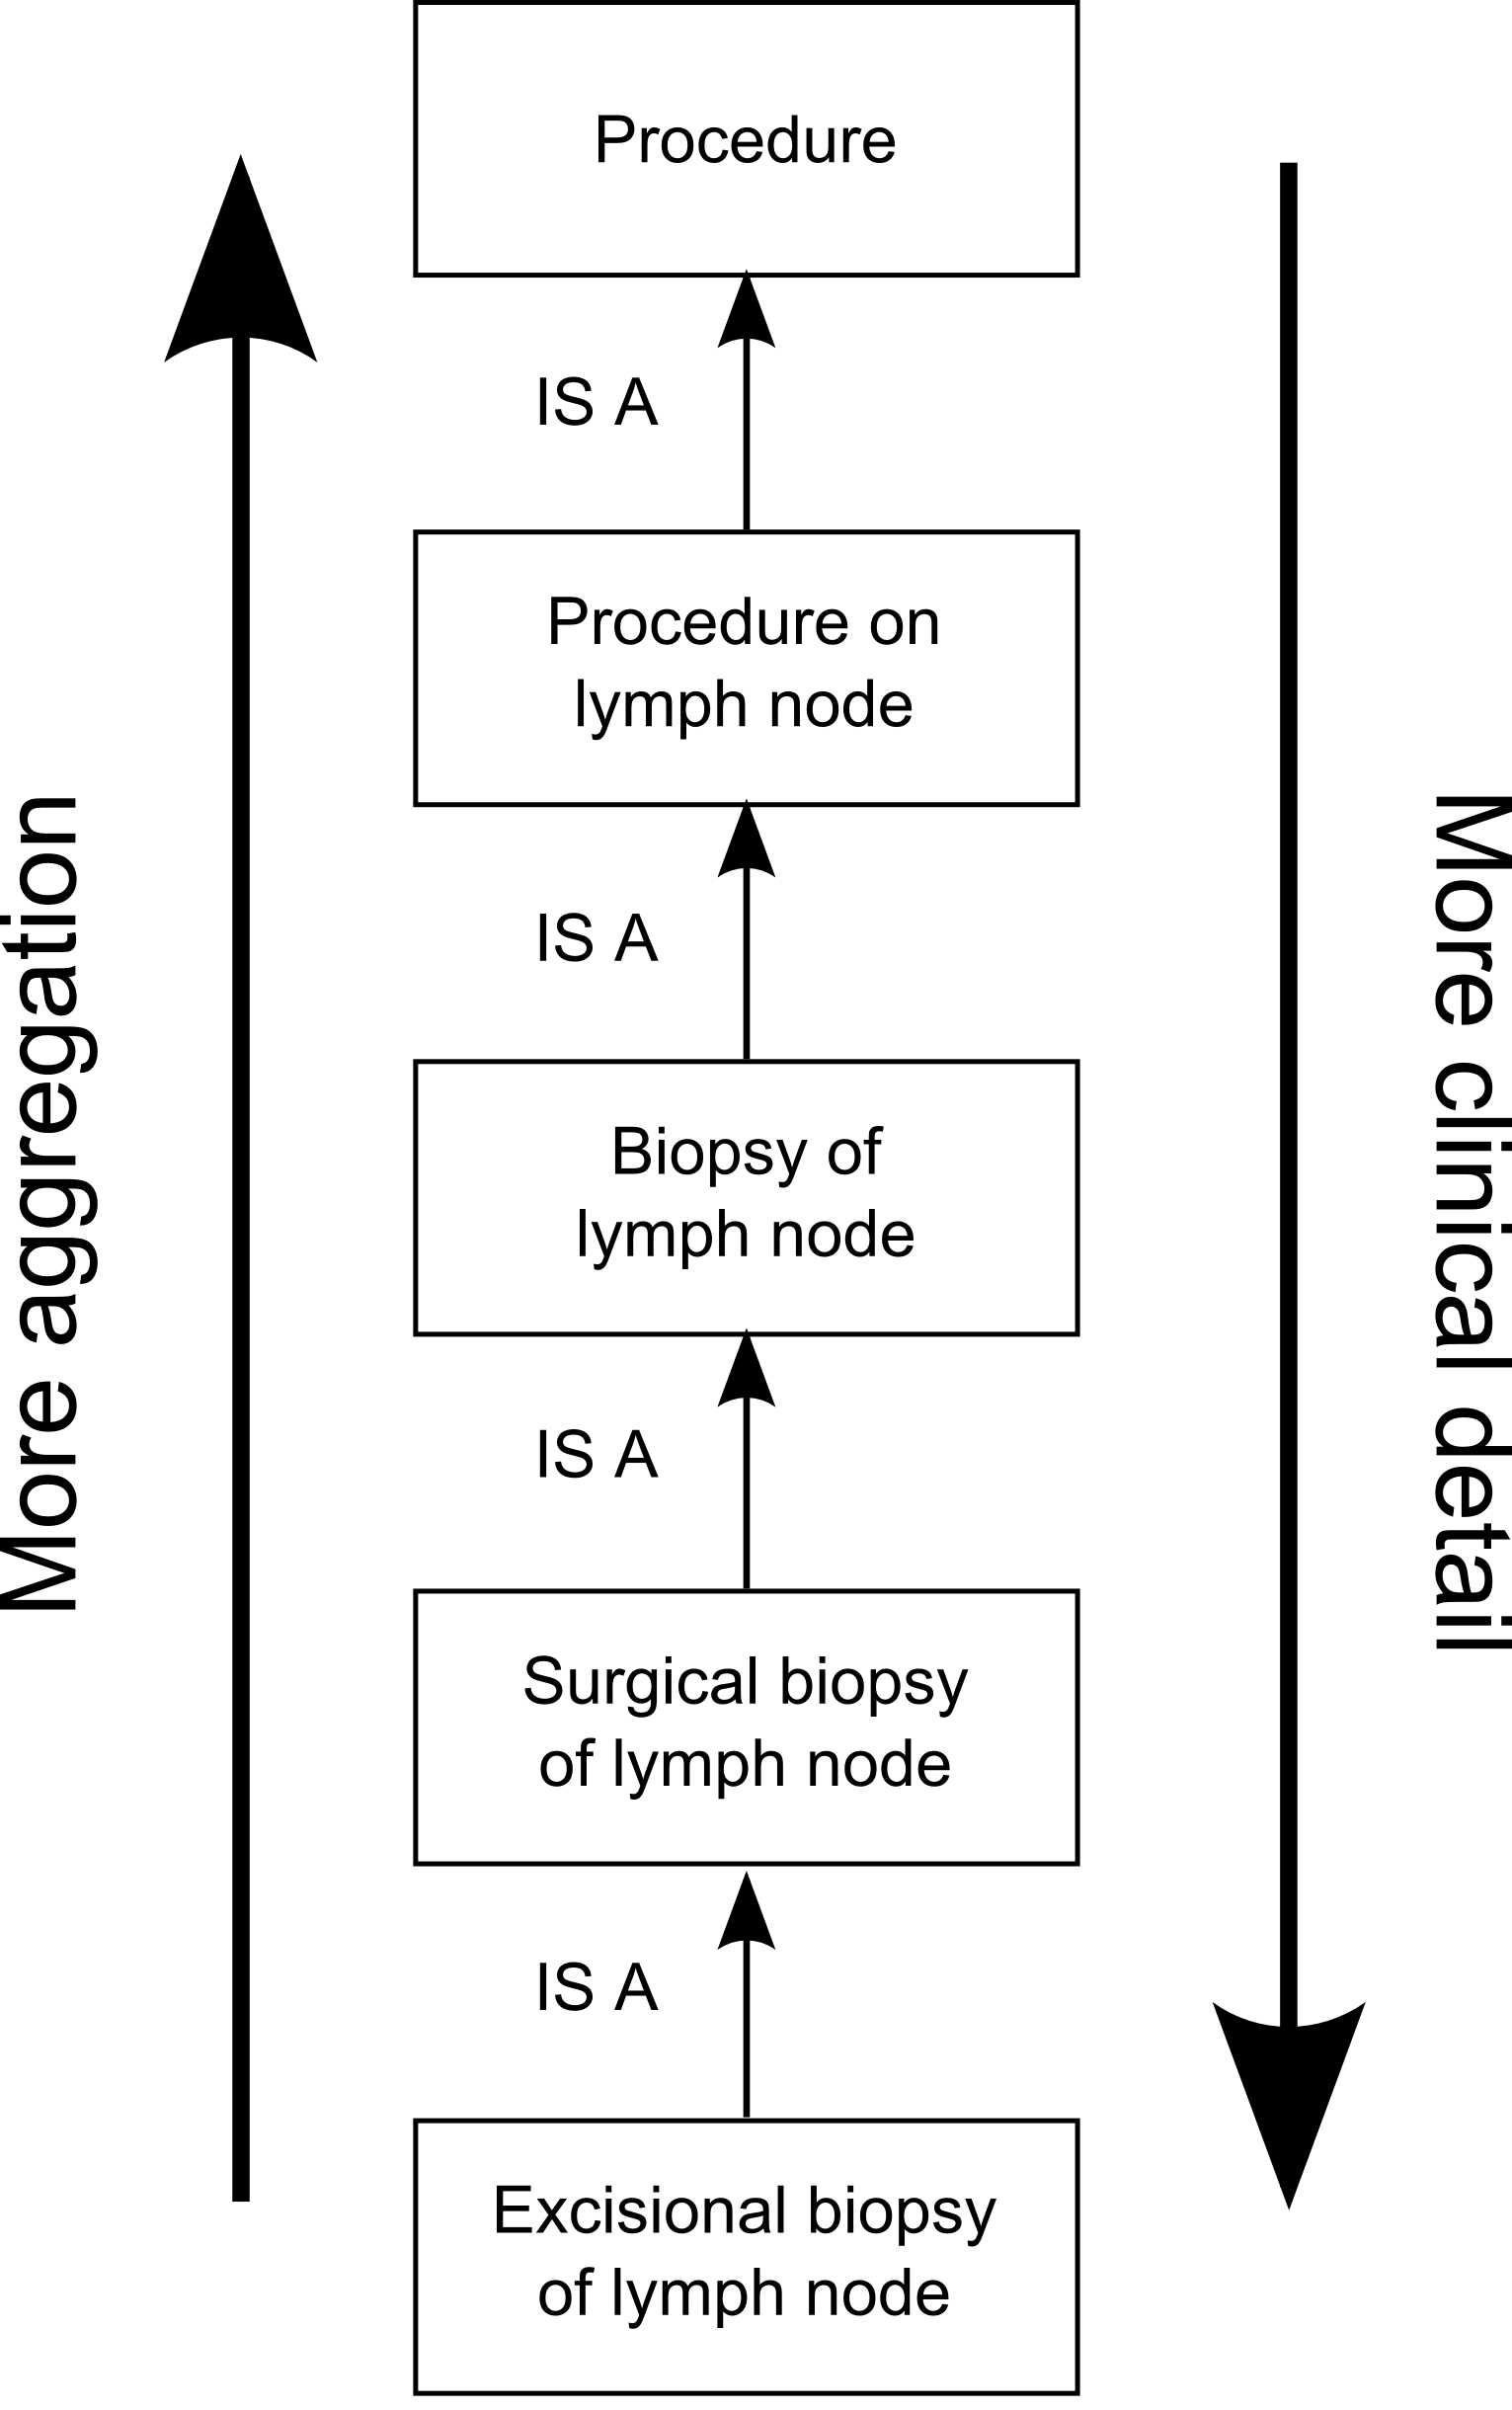
\includegraphics[scale=1]{granularity.png}
    \caption{SNOMED CT - Multiple levels of granularity}\citep[Fig.~1]{snomed_-_user_guide_snomed_2011}
    \label{fig:snomedct_concepts_granularity}
  \end{figure}

  \noindent Concept identifiers in SNOMED CT are meaningless to avoid changes to\
  reflect revised understanding of the nature of a disorder. Meaningless identifiers\
  also enable multiple aspects of meaning to be represented in the same way.\\
  
  \subsection{Descriptions}
  Concept Descriptions are the terms or names assigned to a SNOMED CT concept.\
  A unique DescriptionId  identifies a Description. Multiple Descriptions might be\
  associated with a concept identified by a ConceptId. There are nearly a million\
  English Descriptions in the International Release of SNOMED CT. Each translation\ 
  of SNOMED CT includes an additional set of descriptions, which link terms in another\
  language to the same SNOMED CT concepts.
  
  \noindent\textbf{\emph{Example:}}
  Some of the Descriptions associated with \emph{ConceptId} 22298006:
  \begin{itemize}
    \itemsep0ex
    \item{Fully Specified Name: | Myocardial infarction (disorder) | \emph{DescriptionId}\
    751689013}
    \item{Preferred term: Myocardial infarction \emph{DescriptionId} 37436014}
    \item{Synonym: Cardiac infarction \emph{DescriptionId} 37442013}
    \item{Synonym: Heart attack \emph{DescriptionId} 37443015}
    \item{Synonym: Infarction of heart \emph{DescriptionId} 37441018}
  \end{itemize}
  Each of the above Descriptions has a unique \emph{DescriptionId}, and all of these\
  Descriptions are associated with a single Concept (and the single \emph{ConceptId} 22298006).\\

  \subsection{Relationships}
  SNOMED CT Relationships link each concept to other concepts that have a related\
  meaning. These relationships provide formal definitions and other characteristics of\
  the concept. One type of link is the \textbar ~is a \textbar ~relationship which\
  relates a concept to the its more general concepts. For example (Figure~\ref{fig:snomedct_relationships}), the concept\
  ``viral pneumonia'' has an \textbar ~is a \textbar ~relationship to the more\
  general concept ``pneumonia''. These \textbar ~is a \textbar ~relationships\
  define the hierarchy of SNOMED CT concepts. Other types of relationships\
  represent other aspects of the definition of a concept. For example, the concept\
  ``bacterial pneumonia'' has a \textbar ~causative agent \textbar ~relationship to\
  the concept ``bacteria'' and a \textbar ~finding site \textbar ~relationship to the\
  concept ``lung structure''. There are well over a million relationships in SNOMED CT.
  \begin{figure}[!ht]
    \centering
    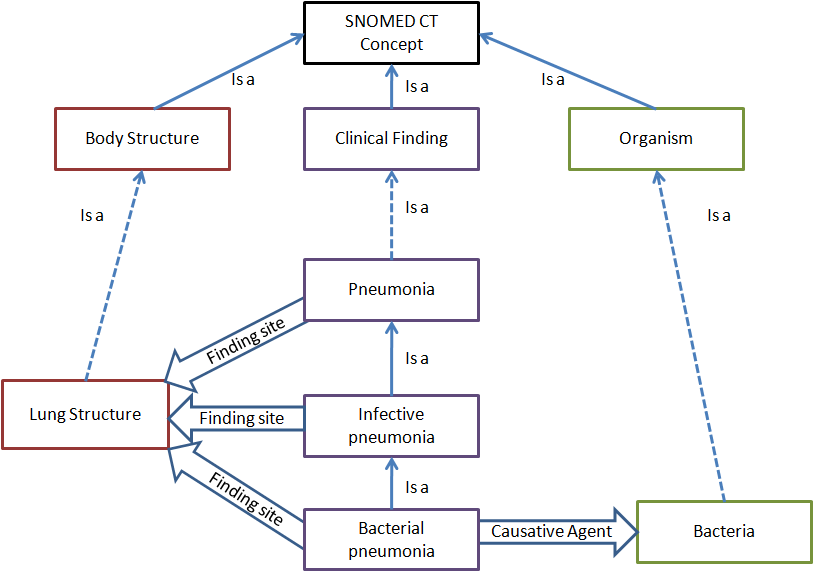
\includegraphics[scale=0.5]{defining_relationship_example1.png}
    \caption{SNOMED CT - Illustration of Defining Relationships}\citep[Fig.~7]{snomed_-_user_guide_snomed_2011}
    \label{fig:snomedct_relationships}
  \end{figure}

\subsection{Implementation}
  SNOMED CT is distributed as a set of tab-delimited text files that can be\
  imported into a relational database. The three tables - the Concepts table,\
  the Descriptions table and the Relationships table are commonly referred to\
  as \emph{Core Components}~\citep{snomed_implementation_guide_snomed_2011}.\
  Supplementary tables called \emph{Reference Sets} specify the common extensible\
  pattern that is used to add additional information related to the core components.

  \subsection{Summary}
  SNOMED CT is a used widely to achieve semantic uniformity\
  and consistency of health terms as well as to achieve interoperability between\
  HL7\textsuperscript{\ref{sec:fhir}}\
  (Health Level 7) based health frameworks and other healthcare entities as shown\
  by the works in \citep{ryan_towards_2006,arguello_executing_2009,khan_achieving_2012}.\
  Not only does it provide unique semantic identifiers to clinical concepts, SNOMED CT\
  also describes and links different concepts in an ontogolical fashion.\
  While SNOMED CT has emerged internationally as a leading terminology, the work of\
  \citep{he_clinical_2012, khare_exploiting_2012} delineates that the existing SNOMED CT\
  lexicon suffers from a surprisingly huge paucity of synonyms.\
  Efforts are underway to reduce SNOMED CT's structural complexity\
  and provide a metathesaurus of clinical concepts with mappings to different terminologies,\
  thereby improving semantic integrity in practical healthcare scenarios.\
  \citep{lindberg_unified_1993,wei_using_2012}
